\documentclass[man]{apa6}
\usepackage{lmodern}
\usepackage{amssymb,amsmath}
\usepackage{ifxetex,ifluatex}
\usepackage{fixltx2e} % provides \textsubscript
\ifnum 0\ifxetex 1\fi\ifluatex 1\fi=0 % if pdftex
  \usepackage[T1]{fontenc}
  \usepackage[utf8]{inputenc}
\else % if luatex or xelatex
  \ifxetex
    \usepackage{mathspec}
  \else
    \usepackage{fontspec}
  \fi
  \defaultfontfeatures{Ligatures=TeX,Scale=MatchLowercase}
\fi
% use upquote if available, for straight quotes in verbatim environments
\IfFileExists{upquote.sty}{\usepackage{upquote}}{}
% use microtype if available
\IfFileExists{microtype.sty}{%
\usepackage{microtype}
\UseMicrotypeSet[protrusion]{basicmath} % disable protrusion for tt fonts
}{}
\usepackage{hyperref}
\hypersetup{unicode=true,
            pdftitle={Reanalysis of Psychological Paper: Computer Game Play Reduces Intrusive Memories of Experimental Trauma via Reconsolidation-Update Mechanisms},
            pdfauthor={Ana-Louise Franz},
            pdfkeywords={reconsolidation, cognitive task},
            pdfborder={0 0 0},
            breaklinks=true}
\urlstyle{same}  % don't use monospace font for urls
\usepackage{graphicx,grffile}
\makeatletter
\def\maxwidth{\ifdim\Gin@nat@width>\linewidth\linewidth\else\Gin@nat@width\fi}
\def\maxheight{\ifdim\Gin@nat@height>\textheight\textheight\else\Gin@nat@height\fi}
\makeatother
% Scale images if necessary, so that they will not overflow the page
% margins by default, and it is still possible to overwrite the defaults
% using explicit options in \includegraphics[width, height, ...]{}
\setkeys{Gin}{width=\maxwidth,height=\maxheight,keepaspectratio}
\IfFileExists{parskip.sty}{%
\usepackage{parskip}
}{% else
\setlength{\parindent}{0pt}
\setlength{\parskip}{6pt plus 2pt minus 1pt}
}
\setlength{\emergencystretch}{3em}  % prevent overfull lines
\providecommand{\tightlist}{%
  \setlength{\itemsep}{0pt}\setlength{\parskip}{0pt}}
\setcounter{secnumdepth}{0}
% Redefines (sub)paragraphs to behave more like sections
\ifx\paragraph\undefined\else
\let\oldparagraph\paragraph
\renewcommand{\paragraph}[1]{\oldparagraph{#1}\mbox{}}
\fi
\ifx\subparagraph\undefined\else
\let\oldsubparagraph\subparagraph
\renewcommand{\subparagraph}[1]{\oldsubparagraph{#1}\mbox{}}
\fi

%%% Use protect on footnotes to avoid problems with footnotes in titles
\let\rmarkdownfootnote\footnote%
\def\footnote{\protect\rmarkdownfootnote}


  \title{Reanalysis of Psychological Paper: Computer Game Play Reduces Intrusive
Memories of Experimental Trauma via Reconsolidation-Update Mechanisms}
    \author{Ana-Louise Franz\textsuperscript{}}
    \date{}
  
\shorttitle{Reanalysis}
\affiliation{
\vspace{0.5cm}
\textsuperscript{1} Brooklyn College}
\keywords{reconsolidation, cognitive task\newline\indent Word count: X}
\usepackage{csquotes}
\usepackage{upgreek}
\captionsetup{font=singlespacing,justification=justified}

\usepackage{longtable}
\usepackage{lscape}
\usepackage{multirow}
\usepackage{tabularx}
\usepackage[flushleft]{threeparttable}
\usepackage{threeparttablex}

\newenvironment{lltable}{\begin{landscape}\begin{center}\begin{ThreePartTable}}{\end{ThreePartTable}\end{center}\end{landscape}}

\makeatletter
\newcommand\LastLTentrywidth{1em}
\newlength\longtablewidth
\setlength{\longtablewidth}{1in}
\newcommand{\getlongtablewidth}{\begingroup \ifcsname LT@\roman{LT@tables}\endcsname \global\longtablewidth=0pt \renewcommand{\LT@entry}[2]{\global\advance\longtablewidth by ##2\relax\gdef\LastLTentrywidth{##2}}\@nameuse{LT@\roman{LT@tables}} \fi \endgroup}


\DeclareDelayedFloatFlavor{ThreePartTable}{table}
\DeclareDelayedFloatFlavor{lltable}{table}
\DeclareDelayedFloatFlavor*{longtable}{table}
\makeatletter
\renewcommand{\efloat@iwrite}[1]{\immediate\expandafter\protected@write\csname efloat@post#1\endcsname{}}
\makeatother
\usepackage{lineno}

\linenumbers

\authornote{

Correspondence concerning this article should be addressed to Ana-Louise
Franz, Postal address. E-mail:
\href{mailto:afranz100@gmail.com}{\nolinkurl{afranz100@gmail.com}}}

\abstract{
There are a few moments in the creation and recollection of memory where
this process can be interrupted. This can be used to help people who are
suffering from the results of tramatic memories. This study examined the
process of reconsolidation, the recollection of a memory, to determine
if there is a way to inturrupt this process using a cognitive task. The
cognitive task used in this experiment was a simple game of Tetris.


}

\begin{document}
\maketitle

\section{Methods}\label{methods}

\subsection{Participants}\label{participants}

52 participants (31 female, 21 males) which consisted of university
students and the general public. 65\% of the participants were students.

\subsection{Material}\label{material}

The details of the trauma exposure and the reconsolidation task are
detailed in James et al. (2015).

\subsection{Procedure}\label{procedure}

The experiment was performed both in the lab and at home in the form of
a diary. They watched a traumatic film and were then assinged to either
the cognitive task group or the no task (control) group.

\section{Results}\label{results}

\begin{figure}
\centering
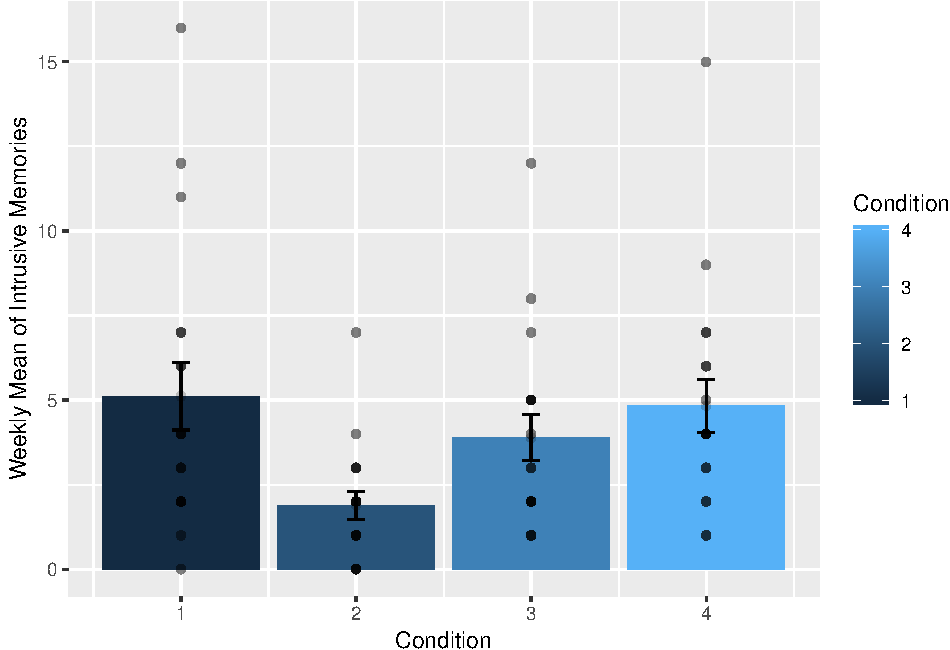
\includegraphics{Midterm_Paper_files/figure-latex/unnamed-chunk-1-1.pdf}
\caption{}
\end{figure}

Using a between subjects one-factor ANOVA, with intervention type as the
independent variable, there was a significant difference between the
different task groups (No-task control, Reactivation Plus tetris, Tetris
only, Reactivation only). There was a main effect of interevention type
\(F(3, 68) = 3.79\), \(\mathit{MSE} = 10.09\), \(p = .014\),
\(\hat{\eta}^2_G = .143\). There was a significant reduction in
traumatic memory reconsolidation for the reactivation and tetris group.

\section{Discussion}\label{discussion}

The omnibus ANOVA that was conducted replicated the results that were
found in James et al. (2015). When traumatic memory reactivation was
interrupted by a cognitive task (tetris) there was an overall reduction
in intrusive memories.

\newpage

\section{Power Analysis}\label{power-analysis}

A power analysis was conducted, and the graph is shown on the final page
of this paper.

\begin{figure}
\centering
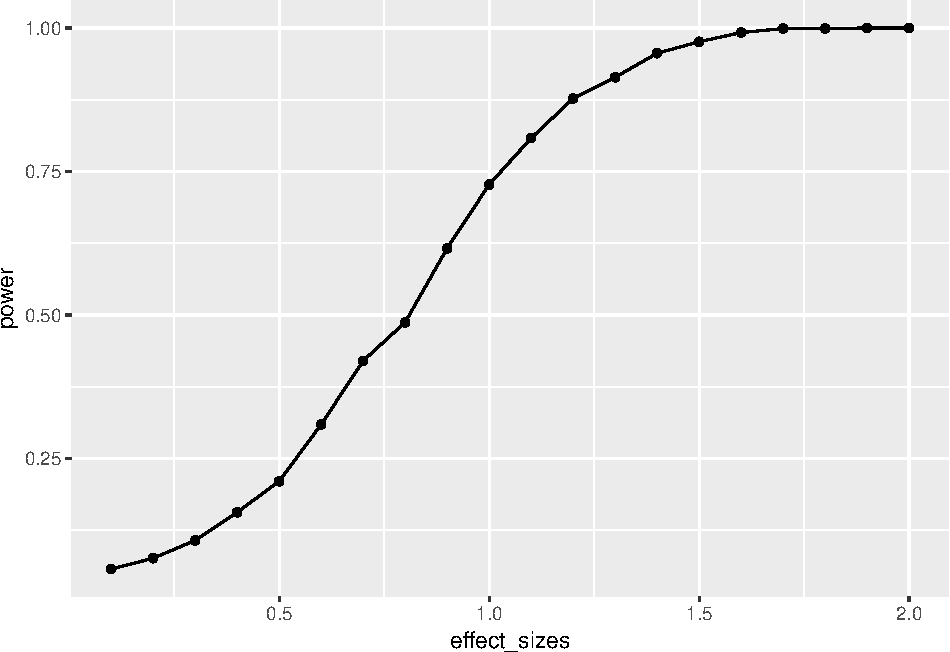
\includegraphics{Midterm_Paper_files/figure-latex/unnamed-chunk-2-1.pdf}
\caption{}
\end{figure}

\section{References}\label{references}

\begingroup
\setlength{\parindent}{-0.5in} \setlength{\leftskip}{0.5in}

\hypertarget{refs}{}
\hypertarget{ref-james2015computer}{}
James, E. L., Bonsall, M. B., Hoppitt, L., Tunbridge, E. M., Geddes, J.
R., Milton, A. L., \& Holmes, E. A. (2015). Computer game play reduces
intrusive memories of experimental trauma via reconsolidation-update
mechanisms. \emph{Psychological Science}, \emph{26}(8), 1201--1215.

\endgroup


\end{document}
